% !TeX root = ../../main.tex
\subsection{Task Outcomes and Observation Cost}
\paragraph{Latest test.}
Table~\ref{tab:latest} reports the selected standard policy on cohort C. It
achieves $70/72$ correct decisions: $50/52$ feasible openings and $20/20$
correct refusals. Learned and always inspection have identical per-scene
opening, refusal, and collision outcomes. Selective inspection reduces the
number of additional inspections by $40.3\%$ ($72\rightarrow43$), mean episode duration
by $31.2\%$ ($55.68\rightarrow38.31$~s), and base travel by $41.7\%$
($4.901\rightarrow2.856$~m). Never inspecting is faster but yields $50/72$
correct decisions, with 20 false refusals. The learned decision preserves
the task performance of obtaining the extra view while avoiding unnecessary
inspection journeys. Figure~\ref{fig:report_cost} visualizes this accuracy--time
comparison for the three inspection modes.

\begin{table}[H]
\caption{Test cohort C: 72 scenes, 52 candidate-feasible and 20
library-infeasible. Time and path are whole-episode means. All rows have zero
observed collisions. The two blocks separate inspection-mode comparison from
the output-retention training ablation.}
\label{tab:latest}
\centering\small
\begin{tabular}{@{}lrrrrrrr@{}}
\toprule
Policy & Open & Correct & False & Inspect & Time & Path & Net \\
 & /52 & /72 & refusal & /72 & (s) & (m) & utility \\
\midrule
\multicolumn{8}{@{}l}{\textit{Inspection modes: same frozen continuation}} \\
Never inspect & 32 & 50 & 20 & 0 & 12.38 & 0.362 & 0.4167 \\
Always inspect & 50 & 70 & 2 & 72 & 55.68 & 4.901 & 0.5136 \\
\textbf{Learned (primary)} & 50 & 70 & 2 & 43 & 38.31 & 2.856 & 0.5853 \\
\midrule
\multicolumn{8}{@{}l}{\textit{Training ablation: output retention}} \\
Retention & 51 & 71 & 1 & 41 & 37.55 & 2.723 & 0.6041 \\
\bottomrule
\end{tabular}
\end{table}

\paragraph{Repeated evaluation of the selected policy.}
Table~\ref{tab:cohorts} summarizes the same policy on three disjoint test
cohorts (A, B, and C). The 54 parameter groups yield $210/216$
correct decisions, $150/153$ feasible openings, $60/63$ correct refusals,
and zero observed collisions. The learned policy uses 125 inspections
versus 216 for always inspecting, with matching per-scene task outcomes in
each cohort.

\begin{table}[tb]
\caption{Same policy on three disjoint 72-scene test cohorts.
``L/A'' gives learned/always inspection.}
\label{tab:cohorts}
\centering\small
\begin{tabular}{@{}lrrrrrr@{}}
\toprule
Cohort & Correct & Open/feasible & Correct refusal & Collisions
 & Inspections L/A & Time L/A (s) \\
\midrule
A & 68/72 & 47/48 & 21/24 & 0 & 43/72 & 37.15/54.46 \\
B & 72/72 & 53/53 & 19/19 & 0 & 39/72 & 37.60/57.55 \\
C & 70/72 & 50/52 & 20/20 & 0 & 43/72 & 38.31/55.68 \\
\midrule
Total & 210/216 & 150/153 & 60/63 & 0 & 125/216 & 37.69/55.90 \\
\bottomrule
\end{tabular}
\end{table}

\ifshowfigures
\begin{figure}[tb]
\centering
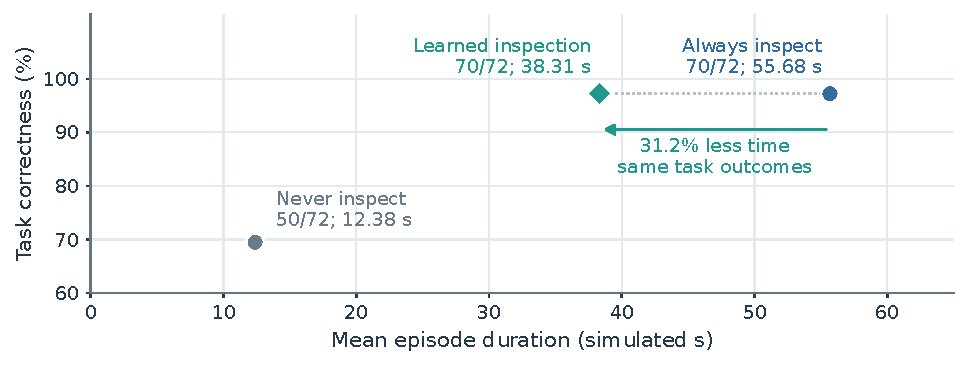
\includegraphics[width=\linewidth]{figures/results/report_inspection_cost.pdf}
\caption{Accuracy--time tradeoff on test cohort C (72 scenes), with the
same P/G continuation for all three inspection modes. Learned inspection
matches always inspecting at $70/72$ correct decisions and reduces mean
episode duration from 55.68 to 38.31 simulated seconds ($31.2\%$).}
\label{fig:report_cost}
\end{figure}
\fi

\Needspace{11\baselineskip}
\begin{samepage}
\paragraph{Controlled inspection-objective study.}
On cohort A, adding the weighted decision term to outcome and cost
supervision reduces inspections from 49 to 43 while retaining $68/72$
correct decisions and identical per-scene task outcomes. Mean duration falls
from 40.86 to 37.15~s, path length from 3.257 to 2.832~m, and net utility
rises from 0.4868 to 0.5015. The pure decision objective uses 42 inspections
but has lower net utility, 0.4901. Outcome supervision thus remains useful
alongside the decision term.
\end{samepage}
